\documentclass[
	aspectratio=169, % default is 43
	8pt, % font size, default is 11pt
	handout, % handout mode without animations, comment out to add animations
]{beamer}

\documentclass[
	aspectratio=169, % default is 43
	8pt, % font size, default is 11pt
	handout, % handout mode without animations, comment out to add animations
]{beamer}

\usepackage{../template/beamerthemeuulm} % use the inofficial uulm beamer theme
\setfaculty{infIngPsy} % set the color scheme for your faculty here [med/infIngPsy/math/nat]

% requires symbolic links
% git clone git@github.com:SoftVarE-Group/SlideTemplate.git C:\Users\...\SlideTemplate
% mklink /J template C:\Users\...\SlideTemplate
% git clone git@spgit.informatik.uni-ulm.de:thuem/slides.git C:\Users\...\ThomasSlides
% mklink /J thomasslides C:\Users\...\ThomasSlides
\graphicspath{{../template/pics/logos}{../template/pics/nature}{../template/pics/uulm}{../thomasslides/}{../pics/}}

%\usepackage[ngerman]{babel} % use this line for slides in German
%\recordingtrue % special recording mode for use with a greenscreen, gives you space to show yourself in a layer in front of the slides, has no effect in the handout mode

\title{Software Product Lines} % short title is used for the slide footer but optional

%
%
%% IMPORTED PACKAGES
%
%\usepackage{adjustbox} % used for partofpage
%\usepackage{tcolorbox} % used for mydefinition, mynote, myexample
\usepackage{multicol} % used temporarily for the lecture overview
%\usepackage{mathtools} % required for absolute value in modeling lecture
%
%% SLIDE TEMPLATE
%
%\beamertemplatenavigationsymbolsempty 
%
%% COMMANDS TO LAYOUT AND ANNIMATE SLIDES
%
\newcommand{\lessonslearned}[3]{
	\subsection{Summary}
	\begin{frame}{\insertsection -- \insertsubsection}
		\leftorright{
			\mydefinition{Lessons Learned}{
				\begin{itemize}
					#1
				\end{itemize}
			}
			\mynote{Further Reading}{
				\small % references take space, can be a little smaller
				\begin{itemize}
					#2
				\end{itemize}
			}
		}{
			\myexample{Practice}{
				#3
			}
		}
	\end{frame}
}

\renewcommand{\lectureoverview}{
%	\section*{Overview}
%	\subsection*{Overview}
	\begin{frame}{\insertsubtitle}
		\begin{multicols}{2}
			\tableofcontents
		\end{multicols}
	\end{frame}
}

%
%\newcommand{\onlyleft}[1]{
%	\halfpage{#1}
%}
%
%\newcommand{\onlyright}[1]{
%	~\hfill
%	\halfpage{#1}
%}
%
%\newcommand{\leftorright}[2]{
%	\uncover<1>{\halfpage{#1}}
%	\hfill
%	\uncover<3->{\halfpage{#2}}
%}
%
%\newcommand{\rightorleft}[2]{
%	\uncover<3->{\halfpage{#1}}
%	\hfill
%	\uncover<1>{\halfpage{#2}}
%}
%
%\newcommand{\leftthenright}[2]{
%	\halfpage{#1}
%	\hfill\pause
%	\halfpage{#2}
%}
%
%\newcommand{\leftandright}[2]{
%	\halfpage{#1}
%	\hfill
%	\halfpage{#2}
%}
%
%\newcommand{\leftmiddleandright}[3]{
%	\thirdpage{#1}
%	\hfill
%	\thirdpage{#2}
%	\hfill
%	\thirdpage{#3}
%}
%
%\newcommand{\leftmiddleorright}[3]{
%	\uncover<1>{\thirdpage{#1}}
%	\hfill
%	\uncover<3>{\thirdpage{#2}}
%	\hfill
%	\uncover<5->{\thirdpage{#3}}
%}
%
%\newcommand{\halfpage}[1]{\partofpage{48}{#1}}
%
%\newcommand{\thirdpage}[1]{\partofpage{31}{#1}}
%
%\newcommand{\partofpage}[2]{
%	\adjustbox{valign=t}{\begin{minipage}{0.#1\textwidth}
%			\begin{flushleft}
%				#2
%			\end{flushleft}
%	\end{minipage}}
%}
%
%\newcommand{\mydefinition}[2]{
%	\begin{tcolorbox}[title=#1,colback=orange!10,colframe=orange!30,coltitle=black,fonttitle=\bfseries,left=1mm,right=1mm,top=1mm,bottom=1mm]
%		\begin{flushleft}
%			#2
%		\end{flushleft}
%	\end{tcolorbox}
%}
%
%\newcommand{\mydefinitiontight}[2]{
%	\begin{tcolorbox}[title=#1,colback=white,colframe=orange!30,coltitle=black,fonttitle=\bfseries,left=0mm,right=0mm,top=0mm,bottom=0mm]
%		\begin{flushleft}
%			#2
%		\end{flushleft}
%	\end{tcolorbox}
%}
%
%\newcommand{\mynote}[2]{
%	\begin{tcolorbox}[title=#1,colback=red!10,colframe=red!30,coltitle=black,fonttitle=\bfseries,left=1mm,right=1mm,top=1mm,bottom=1mm]
%		\begin{flushleft}
%			#2
%		\end{flushleft}
%	\end{tcolorbox}
%}
%
%\newcommand{\myexample}[2]{
%	\begin{tcolorbox}[title=#1,colback=blue!10,colframe=blue!30,coltitle=black,fonttitle=\bfseries,left=1mm,right=1mm,top=1mm,bottom=1mm]
%		\begin{flushleft}
%			#2
%		\end{flushleft}
%	\end{tcolorbox}
%}
%
%\newcommand{\myexampletight}[2]{
%	\begin{tcolorbox}[title=#1,colback=white,colframe=blue!30,coltitle=black,fonttitle=\bfseries,left=0mm,right=0mm,top=0mm,bottom=0mm]
%		\begin{flushleft}
%			#2
%		\end{flushleft}
%	\end{tcolorbox}
%}

\subtitle{4. Feature Modeling}
\author{Elias Kuiter, Thomas Thüm, Timo Kehrer}

\begin{document}

% TITLE SLIDE

\maketitle

% SLIDE TEMPLATE

%\setbeamercolor{title}{fg=black}
%\setbeamercolor{frametitle}{fg=black}
\setbeamertemplate{frametitle}{{\huge~\\\insertsubsection~\insertframetitle}}
\setbeamertemplate{footline}[text line]{\parbox{\linewidth}{\vspace*{-10pt}\hspace{0pt}%
	\insertshortauthor\phantom{g\insertpagenumber}%
	\hfill%
	\inserttitle%
	\ifx \insertsubtitle \empty \else \ -- \insertsubtitle\fi%
	\ifx \insertsectionhead \empty \else \ -- \insertsectionhead\fi%
	\hfill%
	\phantom{g\insertshortauthor}\insertpagenumber%
}}
%\defbeamertemplate{footline}{\begin{beamercolorbox}[sep=1em]{author in head/foot}\insertshortauthor\hfill\insertsection\hfill\insertframenumber\end{beamercolorbox}}
%\defbeamertemplate*{footline}{mytheme}{\begin{beamercolorbox}[sep=1em]{author in head/foot}\insertshortauthor\hfill\insertsection\hfill\insertframenumber\end{beamercolorbox}}

% OVERVIEW SLIDES

\newcommand{\overview}{
	\section*{Overview}
	\subsection*{Overview}
	\begin{frame}{-- \insertsubtitle}
		\begin{multicols}{3}
			\tableofcontents
		\end{multicols}
	
		\begin{flushright}
			\footnotesize
			Author: \insertauthor
			
			Date: \insertdate
		\end{flushright}
	\end{frame}
}
% temporarily added slide to have a lecture overview 
\overview

% temporarily removed
%\begin{frame}{Lecture Overview -- \insertsubtitle}
%	\tableofcontents[hideallsubsections]
%\end{frame}

\AtBeginSection[]{%
	\begin{frame}{Lecture Overview -- \insertsubtitle}
		\tableofcontents[currentsection,hideothersubsections]
	\end{frame}
}

\newcommand{\sectionend}{\addtocontents{toc}{\newpage}}


\section{Feature Models}

\subsection{Recap: Software Product Lines}
\begin{frame}{\myframetitle}
	\begin{mycolumns}
		\mydefinition{Software Product Line \mysource{\seiwhitepaperspl\mypage{5}}}{\mycitebegin A \emph{software product line} is 
			\begin{itemize}
				\item a set of software-intensive systems
				\item that share a common, managed set of features
				\item satisfying the specific needs of a particular market segment or mission
				\item and that are developed from a common set of core assets in a prescribed way.\myciteend
				\mysource{\href{https://resources.sei.cmu.edu/library/asset-view.cfm?assetID=513819}{Software Engineering Institute, Carnegie Mellon University}}
			\end{itemize}
		}
	\mynextcolumn
		\mydefinition{Feature \mysource{\fospl\mypage{18}}}{
			\mycite{A \emph{feature} is a characteristic or end-user-visible behavior of a software system.}
		}
		\mydefinition{Product \mysource{\fospl\mypage{19}}}{
			\mycite{A \emph{product of a product line} is specified by a valid feature selection (a subset of the features of the product line). A feature selection is \emph{valid} if and only if it fulfills all feature dependencies.}
		}
	\end{mycolumns}
\end{frame}

\subsection{Understanding Features and Their Dependencies}

\begin{frame}{\myframetitle}
	\begin{mycolumns}[columns=3,widths={40,20,40}]
		\myexampletight{Ordering a Waffle \ldots}{
			\pic[width=\textwidth]{waffle-feature-model}
		}
		\mynextcolumn
		\myexampletight{\ldots with Sugar}{
			\pic[width=\textwidth]{waffle-sugar}
		}
		\myexampletight{\ldots with Cherries}{
			\pic[width=\textwidth]{waffle-cherries}
		}
		\mynextcolumn
		\mynote{This is Nice, But \ldots}{
			\begin{itemize}
				\item plate and sugar seem to always be included, a fork is only included for some orders\\
					$\Rightarrow$ limitations seem arbitrary
				\item children get special treatment\\
					$\Rightarrow$ order process is unfair
				\item what exactly am I paying for?\\
					$\Rightarrow$ investments are unclear
				\end{itemize}
		}
		\mydefinition{In This Lecture}{
			\begin{enumerate}
				\item how to model and configure features and their dependencies?
				\item how to store and communicate?
				\item how to analyze and understand?
			\end{enumerate}
		}
	\end{mycolumns}
\end{frame}

\xkcdframe{2369}

\subsection{Configurations}

\newcommand{\feat}[1]{{\emph{#1}}}

\begin{frame}{\myframetitle}
	\begin{mycolumns}
		\mydefinition{Configuration}{
			\begin{itemize}
				\item a \emph{configuration} \deutsch{Konfiguration} over a set of features $F$ selects and deselects features in $F$
				\item formally: a pair $(S, D)$ such that $S, D \subseteq F$ and $S, D$ are disjoint ($S \cap D = \varnothing$)
				\item is \emph{complete} \deutsch{vollständig} if all features are covered ($S \cup D = F$) and \emph{partial} \deutsch{partiell} otherwise
				\item a complete configuration is \emph{valid} \deutsch{gültig} if it ``makes sense'' in the domain and \emph{invalid} \deutsch{ungültig} otherwise
				\item we often abbreviate complete configurations with $S \equiv (S, F \setminus S)$
			\end{itemize}
		}
	\mynextcolumn
		\myexample{}{
			\vspace*{-4ex}
			\begin{align*}
				\text{Feature set } F = \{&ConfigDB, Get, Put, Delete,\\
				&Transactions, Windows, Linux\}
			\end{align*}
			Examples for \emph{complete} configurations:
			\begin{itemize}
				\item \emph{valid} (read-only database on Windows):
					$\cfg{C, G, W}{P, D, T, L}$
				\item \emph{valid} (fully functional database on Linux):
					$\cfg{C, G, P, D, T, L}{W}$
				\item \emph{invalid} ($\lightning$ no operating system):
					$\cfg{C, G}{P, D, T, W, L}$
				\item \emph{invalid} (transactions $\lightning$ read-only database):
					$\cfg{C, G, T, L}{P, D, W}$
			\end{itemize}
			Examples for \emph{partial} configurations:
			
			$\cfg{C, G}{P, D}$, $(\varnothing, \varnothing)$
		}
	\end{mycolumns}
\end{frame}

\subsection{Characterizing Valid Configurations}

\subsubsection*{Natural Language}

\begin{frame}{\myframetitle}\label{frame:natlang}
	\begin{mycolumns}
		\mynote{Valid Configuration}{
			A complete configuration over $F$ is valid if it ``makes sense'' in the domain.
			\emph{\color{red}{$\leadsto$ ``makes sense''?}}
		}

		\mydefinition{Natural Language}{
			\begin{itemize}
				\item informal description of relationships between features in $F$
				\item a complete configuration $S$ is \emph{valid} if it conforms to the description
				\item[+] succinct
				\item[--] sometimes ambiguous
				\item[--] not machine-readable
			\end{itemize}
		}
	\mynextcolumn
		\myexample{}{
			``A \feat{configurable database} has an API that allows for at least one of the request types \feat{Get}, \feat{Put}, or \feat{Delete}.
			Optionally, the database can support \feat{transactions}, provided that the API allows for Put or Delete requests.
			Also, the database targets a supported operating system, which is either \feat{Windows} or \feat{Linux}.''
		}
	\end{mycolumns}
\end{frame}

\subsubsection*{Configuration Map}

\begin{frame}{\myframetitle}\label{frame:cfgmap}
	\begin{mycolumns}
		\mynote{Valid Configuration}{
			A complete configuration over $F$ is valid if it ``makes sense'' in the domain.
			\emph{\color{red}{$\leadsto$ ``makes sense''?}}
		}

		\mydefinition{Configuration Map}{
			\begin{itemize}
				\item a \emph{configuration map} over $F$ is a set of complete configurations $C \subseteq F$
				\item a complete configuration $S$ is \emph{valid} if it occurs in the configuration map ($S \in C$)
				\item also known as product map
				\item[+] precise
				\item[--] not human-readable
				\item[--] redundant, explodes in size ($0 \leq \abs{C} \leq 2^{\abs{F}}$)
			\end{itemize}
		}
	\mynextcolumn
		\myexample{}{
			\vspace*{-4ex}
			\begin{align*}
				\text{Feature set } F = \{&ConfigDB, Get, Put, Delete,\\
				&Transactions, Windows, Linux\}
			\end{align*}
			
			Configuration map:
			
			\small
			\leftandright{
				{\color{black}$\{C,G,W\}$}\\
				$\{C,P,W\}$\\
				$\{C,G,P,W\}$\\
				$\{C,D,W\}$\\
				$\{C,G,D,W\}$\\
				$\{C,P,D,W\}$\\
				$\{C,G,P,D,W\}$\\
				$\{C,P,T,W\}$\\
				$\{C,G,P,T,W\}$\\
				$\{C,D,T,W\}$\\
				$\{C,G,D,T,W\}$\\
				$\{C,P,D,T,W\}$\\
				$\{C,G,P,D,T,W\}$
			}{
				$\{C,G,L\}$\\
				$\{C,P,L\}$\\
				$\{C,G,P,L\}$\\
				$\{C,D,L\}$\\
				$\{C,G,D,L\}$\\
				$\{C,P,D,L\}$\\
				$\{C,G,P,D,L\}$\\
				$\{C,P,T,L\}$\\
				$\{C,G,P,T,L\}$\\
				$\{C,D,T,L\}$\\
				$\{C,G,D,T,L\}$\\
				$\{C,P,D,T,L\}$\\
				{\color{black}$\{C,G,P,D,T,L\}$}
			}
		}
	\end{mycolumns}
\end{frame}

\subsubsection*{Excel}

\begin{frame}{\myframetitle}
	\centering
	\includegraphics[width=0.48\linewidth]{products-in-excel}

	\textbf{Can we do better?}
\end{frame}

\subsection{Feature Models}

\subsubsection*{Syntax}

\begin{frame}{\myframetitle\ \mytitlesource{\fospl; \foda\mypages{63--72}; \batorygrammars}}
	\begin{mycolumns}
		\myexampletight{}{
			\centering
			\featureDiagramConfigurableDatabase
			
			\featureDiagramLegend
		}
	\mynextcolumn
		\mydefinition{Feature Model \deutsch{Feature-Modell}}{
			\begin{itemize}
				\item hierarchy of features
				\item dependencies between features modeled by tree and cross-tree constraints
				\item \emph{tree constraints}: defined by the hierarchy
				\item \emph{cross-tree constraints}: propositional formulas over features
				\item \emph{abstract features} are used to group other features
				\item \emph{concrete features} have an implementation
				\item also known as feature diagram or feature tree
				\item notation for \emph{optional/mandatory features} and \emph{or/alternative groups}
			\end{itemize}
		}
	\end{mycolumns}
\end{frame}

\subsubsection*{Semantics}

\begin{frame}{\myframetitle\ \mytitlesource{\fospl; \batorygrammars}}
	\begin{mycolumns}[animation=none]
		\uncover<2-|handout:1>{
			\mydefinition{Tree Constraints}{
				\begin{itemize}
					\item the \emph{root feature} is always required
					\item each feature requires its parent
					\item an \emph{optional feature} can be (de-)selected freely when its parent is selected
					\item a \emph{mandatory feature} is required by its parent
					\item \emph{or group}: at least one feature must be selected when the parent is selected
					\item \emph{alternative group}: exactly one feature must be selected when the parent is selected
				\end{itemize}
			}
		}
	\mynextcolumn
		\myexampletight{}{
			\centering
			\featureDiagramConfigurableDatabase
		}
		\uncover<3|handout:1>{
			\mydefinition{Cross-Tree Constraints}{
				\begin{itemize}
					\item a list of \emph{propositional formulas} expressing further dependencies between features
					\item each cross-tree constraint must be satisfied
				\end{itemize}
			}
		}
	\end{mycolumns}
\end{frame}

\subsubsection*{Examples}

\begin{frame}{\myframetitle}
	\begin{mycolumns}[animation=none]
		\myexampletight{}{
			\centering
			\featureDiagramConfigurableDatabase[_fm]
			\featureDiagramOverlay{
				\only<2|handout:0>{
					\featureSelected{(ConfigDB_fm),(API_fm),(Get_fm),(OS_fm),(Windows_fm)}
					\featureDeselected{(Put_fm)(Delete_fm),(Transactions_fm),(Linux_fm)}
				}
				\only<3|handout:0>{
					\featureSelected{(ConfigDB_fm),(API_fm)(Transactions_fm)(OS_fm),(Get_fm)(Put_fm)(Delete_fm),(Linux_fm)}
					\featureDeselected{(Windows_fm)}
				}
				\only<4|handout:0>{
					\featureSelected{(ConfigDB_fm),(API_fm),(Get_fm)}
					\featureDeselected{(Put_fm)(Delete_fm)(Windows_fm)(Linux_fm),(Transactions_fm)(OS_fm)}
				}
				\only<5|handout:0>{
					\featureSelected{(ConfigDB_fm),(API_fm)(Transactions_fm)(OS_fm),(Get_fm),(Linux_fm)}
					\featureDeselected{(Put_fm)(Delete_fm)(Windows_fm)}
				}
			}
		}
	\mynextcolumn
		\myexample{Is This a Valid Configuration?}{
			\begin{itemize}
				\item<2-|handout:1> \emph{valid} (read-only database on Windows):
					$\cfg[2|handout:0]{C, A, G, O, W}{P, D, T, L}$
				\item<3-|handout:1> \emph{valid} (fully functional database on Linux):
					$\cfg[3|handout:0]{C, A, G, P, D, T, O, L}{W}$
				\item<4-|handout:1> \emph{invalid} ($\lightning$ no operating system):
					$\cfg[4|handout:0]{C, A, G}{P, D, T, O, W, L}$
				\item<5-|handout:1> \emph{invalid} (transactions $\lightning$ read-only database):
					$\cfg[5|handout:0]{C, A, G, T, O, L}{P, D, W}$
			\end{itemize}
		}
	\end{mycolumns}
\end{frame}

\begin{frame}{\myframetitle}
	\begin{mycolumns}[columns=3,widths={5,90,5}]
	\mynextcolumn
		\myexampletight{}{
			\centering
			\featureDiagramWaffle
			% sugar is false-optional
			% implicit constraint: cherries implies adult
		}
	\mynextcolumn
	\end{mycolumns}

	\begin{mycolumns}[columns=3,widths={5,90,5}]
	\mynextcolumn
		\mynote{A Few Remarks on Notation}{
			\begin{itemize}
				\item abstract and concrete features can be assigned arbitrarily
				\item groups can be used anywhere
				\item directly below groups, no optional or mandatory markers are allowed
			\end{itemize}
		}
	\mynextcolumn
	\end{mycolumns}
\end{frame}

\subsection{Advantages of Feature Modeling}

\begin{frame}{\myframetitle}
	\begin{mycolumns}
		\textbf{Making Tacit Knowledge Explicit}
		\mynote{Interview with Practitioners \mysource{\href{https://link.springer.com/chapter/10.1007/978-3-319-11653-2_19}{Berger~et~al.~2014}}}{
			\mycite{I think the best [about feature modeling] is you can see relationships, to actually know what configurations are allowed and what are not allowed. That was also not so easy to express in the past [\ldots] This is from the developer's point of view. But it's also, we can see that from the, say project development, it's also important, because before we noticed that \emph{the same functionality was implemented twice} within the same project, basically they haven't realized that. They implemented the same features.}
		}
	\mynextcolumn
		\textbf{Tool Support}

		\pic[width=\linewidth]{featureide-feature-model-editor}
	\end{mycolumns}
\end{frame}

\lessonslearned{
	\item features, dependencies between features, configurators
	\item feature models: abstract and concrete features, tree and cross-tree constraints
	\item tree constraints: optional, mandatory, or group, alternative group
}{
	\item \fospl, Section~2.3 Feature Modeling
	\item Thorsten Berger et al. (2013): \href{https://doi.org/10.1145/2430502.2430513}{A Survey of Variability Modeling in Industrial Practice}
	\item Damir Nešić et al. (2019): \href{https://doi.org/10.1145/3338906.3338974}{Principles of Feature Modeling}
}{
	\item sketch a feature model with \todo{X} configurations (pen and paper preferred)
	\item upload your solution to \todots
	\item discuss whether your solutions are syntactically correct and have the right number of configurations
}

\sectionend

\section{Representations and Translations}

\subsection{Representations of Variability Models}

\begin{frame}{\myframetitle} % show list of cfgs, diagrams, text => what are the problems? 
	% this notation is already nice for communication, but semantics matter (for large models, it does not suffice to look sharply)

	% why is this needed? (forward ref?)

	% this section shall teach the relationship between FMs and formulas and FMs and sets (i.e., Damiani 2020, Batory 2005), so: FM semantics

	% also, (valid) total configurations should be explained here (how a computer can check them, this can be checked easily when an FM is encoded eg as runtime variability, but all other SAT-based questions are hard to answer)

	\begin{mycolumns}
		\myexample{Natural Language}{
			\tiny ``A \feat{configurable database} has an API that allows for at least one of the request types \feat{Get}, \feat{Put}, or \feat{Delete}.
			Optionally, the database can support \feat{transactions}, provided that the API allows for Put or Delete requests.
			Also, the database targets a supported operating system, which is either \feat{Windows} or \feat{Linux}.''
		}
		\myexample{Configuration Map}{
			\tiny
			\leftandright{
				$\{C,G,W\}$\\
				\hspace{4mm}\vdots\\[1ex]
				$\{C,G,P,D,T,W\}$
			}{
				$\{C,G,L\}$\\
				\hspace{4mm}\vdots\\[1ex]
				$\{C,G,P,D,T,L\}$
			}
		}
		\myexampletight{Feature Model}{
			\centering\tiny
			\featureDiagramConfigurableDatabase
		}
	\mynextcolumn
		\centering
		\includegraphics[width=\linewidth]{representations-high-level}

		\mynote{Problems}{
			\begin{enumerate}
				\item[P1] How to express feature models \emph{textually}? % animate P1 with arrows, see lego example
				\item[P2] How to obtain configurations \emph{automatically}? % valid cfg
				\item[P3] \color{gray}{(How to reverse engineer feature models?)}
			\end{enumerate}
		}
	\end{mycolumns}
\end{frame}

\subsection{Universal Variability Language}

\begin{frame}[fragile]{\myframetitle}
	\begin{mycolumns}
\begin{uvl}[basicstyle=\normalsize]
features
	ConfigDB	
		mandatory
			API {abstract}
				or
					Get
					Put
					Delete

		optional
			Transactions
		mandatory
			OS {abstract}
				alternative
					Windows
					Linux
				
constraints
	Transactions => Put | Delete
\end{uvl}
	\mynextcolumn
		\myexampletight{A Feature Model ``Sideways''}{
			\centering
			\includegraphics[width=\linewidth]{varied-model}
			$Transactions \pimplies Put \por Delete$
		}
		\mynote{Universal Variability Language (UVL)}{
			\begin{itemize}
				\item textual language for feature modeling
				\item adds advanced modeling constructs (e.g., attributes, cardinalities, submodels, \ldots)
			\end{itemize}
		}
	\end{mycolumns}
\end{frame}

\begin{frame}{\myframetitle}
	\centering
	\includegraphics[width=0.45\linewidth]{representations-high-level}
	\begin{mycolumns}[animation=none]
		\mynote{Problems}{
			\begin{enumerate}
				\item[P1] How to express feature models \emph{textually}?
				\item[P2] How to obtain configurations \emph{automatically}?
				\item[P3] \color{gray}{(How to reverse engineer feature models?)}
			\end{enumerate}
		}
		\mynextcolumn
		\mynote{Solutions}{
			\begin{enumerate}
				\item[P1] Universal Variability Language $\rightarrow$ \emph{Syntax}
				\item[P2] \emph{Semantics}?
				\item[P3] \color{gray}{--}
			\end{enumerate}
		}
	\end{mycolumns}
\end{frame}

\subsection{Recap: Propositional Formulas}

\begin{frame}{\myframetitle}
	\begin{mycolumns}
		\mydefinition{Syntax of Propositional Formulas}{
			Inductive definition of \emph{(propositional) formulas}\\\deutsch{(aussagenlogische) Formeln}:
			\begin{itemize}
				\item the \emph{(Boolean) truth values} $\top$, $\bot$
				\item any \emph{(Boolean) variable} $X$
    			\item any \emph{negation} $\pnot \phi$ of a formula $\phi$
    			\item any \emph{conjunction} $(\phi \pand \psi)$ of formulas $\phi$ and $\psi$
				\item any \emph{disjunction} $(\phi \por \psi)$, \emph{implication} $(\phi \pimplies \psi)$, or \emph{biimplication} $(\phi \pequals \psi)$
			\end{itemize}
		}
		\mynote{Operator Precedence: $\pnot$, $\pand$, $\por$, $\pimplies$, $\pequals$}{
			\vspace*{-4ex} % TODO Benno: why is this hack needed?
			\begin{align*}
				           &~Transactions \pimplies (Put \por Delete) \\
				\equiv     &~Transactions \pimplies Put \por Delete \\
				\not\equiv &~(Transactions \pimplies Put) \por Delete
			\end{align*}
		}
	\mynextcolumn
		\mydefinition{Informal Semantics of Propositional Formulas}{
			\vspace*{-4ex}
			\begin{equation*}
				\begin{rcases}
					\top                \\
					\bot                \\
					\pnot \phi          \\
					\phi \pand \psi     \\
					\phi \por \psi      \\
					\phi \pimplies \psi \\
					\phi \pequals \psi
				\end{rcases} \text{ means } \begin{cases}
					\text{``true'' (or \emph{tautology})} \\
					\text{``false'' (or \emph{contradiction})} \\
					\text{``not $\phi$''} \\
					\text{``$\phi$ and $\psi$''} \\
					\text{``$\phi$ or $\psi$'' (inclusive or!)} \\
					\text{``if $\phi$, then $\psi$'' (and else?)} \\
					\text{``$\phi$ if and only if $\psi$''}
				\end{cases}
			\end{equation*}
		}
		\mynote{Differences to First-Order Logic}{
			\begin{itemize}
				\item no quantifiers $\forall, \exists$
    			\item no predicates $P(\ldots)$ (e.g., $=$, $>$, $isA$)
    			\item no functions $f(\ldots)$ (e.g., $+$, $\ast$, $typeOf$)
				\item no constants (e.g., $42$, ``hello'')
			\end{itemize}
		}
	\end{mycolumns}
\end{frame}

\subsection{From Feature Model to Formula}

\subsubsection{Example}

\begin{frame}{\myframetitle}
	\begin{mycolumns}
		\only<1-|handout:1>{
			\myexampletight{A Feature Model $FM$ \ldots}{
				\centering\tiny
				\featureDiagramConfigurableDatabase[_phi]
				\featureDiagramOverlay{
					\only<1>{
						\featureDeemph{(API_phi),(Get_phi),(Put_phi),(Delete_phi),(Transactions_phi),(OS_phi),(Windows_phi),(Linux_phi)}
						\featureEmph{(ConfigDB_phi)}
					}
					\only<2>{
						\featureDeemph{(Get_phi),(Put_phi),(Delete_phi),(Transactions_phi),(OS_phi),(Windows_phi),(Linux_phi)}
						\featureEmph{(ConfigDB_phi)(API_phi)}
					}
					\only<3>{
						\featureDeemph{(Get_phi),(Put_phi),(Delete_phi),(API_phi),(OS_phi),(Windows_phi),(Linux_phi)}
						\featureEmph{(ConfigDB_phi)(Transactions_phi)}
					}
					\only<4>{
						\featureDeemph{(Get_phi),(Put_phi),(Delete_phi),(API_phi),(Transactions_phi),(Windows_phi),(Linux_phi)}
						\featureEmph{(ConfigDB_phi)(OS_phi)}
					}
					\only<5>{
						\featureDeemph{(ConfigDB_phi),(Transactions_phi),(Windows_phi),(Linux_phi),(OS_phi)}
						\featureEmph{(Get_phi)(Put_phi)(Delete_phi)(API_phi)}
					}
					\only<6-7>{
						\featureDeemph{(Get_phi),(Put_phi),(Delete_phi),(API_phi),(Transactions_phi),(ConfigDB_phi)}
						\featureEmph{(Windows_phi)(Linux_phi)(OS_phi)}
					}
					\only<8>{
						\featureDeemph{(ConfigDB_phi)(Transactions_phi)(Windows_phi)(Linux_phi)(OS_phi)(Get_phi)(Put_phi)(Delete_phi)(API_phi)}
					}
					\only<9-12>{
						\featureSelected{(ConfigDB_phi),(API_phi),(Get_phi),(OS_phi),(Windows_phi)}
						\featureDeselected{(Put_phi)(Delete_phi),(Transactions_phi),(Linux_phi)}
					}
					\only<13->{
						\featureSelected{(ConfigDB_phi),(API_phi),(Get_phi)}
						\featureDeselected{(Put_phi)(Delete_phi)(Windows_phi)(Linux_phi),(Transactions_phi)(OS_phi)}
					}
				}
			}
			\myexample{\ldots as a Propositional Formula $\phi(FM)$}{
				\vspace*{-4ex}
				\small
				\begin{align*}
					\phi(FM) = &~ConfigDB \\
					\uncover<2->{\pand &~(API \pequals ConfigDB) \\}
					\uncover<3->{\pand &~(Transactions \pimplies ConfigDB) \\}
					\uncover<4->{\pand &~(OS \pequals ConfigDB) \\}
					\uncover<5->{\pand &~(Get \por Put \por Delete \pequals API) \\}
					\uncover<6->{\pand &~(Windows \por Linux \pequals OS) \\}
					\uncover<7->{\pand &~\pnot (Windows \pand Linux) \\}
					\uncover<8->{\pand &~(Transactions \pimplies Put \por Delete)}
				\end{align*}
			}
		}
	\mynextcolumn
		\only<9-|handout:2>{
			\myexample{Is This a Valid Configuration?}{
				\vspace*{-4ex}
				\only<9-12>{
					\begin{align*}
								&~\phi(FM)({\{C, A, G, O, W\}}) \\
						=		&~\phi(FM)(\cfg[2-]{C, A, G, O, W}{P, D, T, L}) \\
						\uncover<10->{=&~\fs{C} \pand (\fs{A} \pequals \fs{C}) \pand (\fd{T} \pimplies \fs{C}) \pand (\fs{O} \pequals \fs{C}) \\
						\pand &~(\fs{G} \por \fd{P} \por \fd{D} \pequals \fs{A}) \pand (\fs{W} \por \fd{L} \pequals \fs{O}) \\
						\pand &~\pnot (\fs{W} \pand \fd{L}) \pand (\fd{T} \pimplies \fd{P} \por \fd{D}) \\}
						\uncover<11->{=&~\fs{\top} \pand (\fs{\top} \pequals \fs{\top}) \pand (\fd{\bot} \pimplies \fs{\top}) \pand (\fs{\top} \pequals \fs{\top}) \\
						\pand &~(\fs{\top} \por \fd{\bot} \por \fd{\bot} \pequals \fs{\top}) \pand (\fs{\top} \por \fd{\bot} \pequals \fs{\top}) \\
						\pand &~\pnot (\fs{\top} \pand \fd{\bot}) \pand (\fd{\bot} \pimplies \fd{\bot} \por \fd{\bot}) \\}
						\uncover<12->{=&~\fs{\top} \pand \fs{\top} \pand \fs{\top} \pand \fs{\top} \pand \fs{\top} \pand \fs{\top} \pand \fs{\top} \pand \fs{\top} \\
						=		&~\fs{\top}}
					\end{align*}
					\uncover<12->{\emph{$\leadsto$ configuration is valid}\\
					\phantom{$\leadsto$ }(read-only database on Windows)}
				}
				\only<13->{
					\begin{align*}
								&~\phi(FM)({\{C, A, G\}}) \\
						=		&~\phi(FM)(\cfg[2-]{C, A, G}{P, D, T, O, W, L}) \\
						\uncover<14->{=&~\fs{C} \pand (\fs{A} \pequals \fs{C}) \pand (\fd{T} \pimplies \fs{C}) \pand (\fd{O} \pequals \fs{C}) \\
						\pand &~(\fs{G} \por \fd{P} \por \fd{D} \pequals \fs{A}) \pand (\fd{W} \por \fd{L} \pequals \fd{O}) \\
						\pand &~\pnot (\fd{W} \pand \fd{L}) \pand (\fd{T} \pimplies \fd{P} \por \fd{D}) \\}
						\uncover<15->{=&~\fs{\top} \pand (\fs{\top} \pequals \fs{\top}) \pand (\fd{\bot} \pimplies \fs{\top}) \pand (\fd{\bot} \pequals \fs{\top}) \\
						\pand &~(\fs{\top} \por \fd{\bot} \por \fd{\bot} \pequals \fs{\top}) \pand (\fd{\bot} \por \fd{\bot} \pequals \fd{\bot}) \\
						\pand &~\pnot (\fd{\bot} \pand \fd{\bot}) \pand (\fd{\bot} \pimplies \fd{\bot} \por \fd{\bot}) \\}
						\uncover<16->{=&~\fs{\top} \pand \fs{\top} \pand \fs{\top} \pand \fd{\bot} \pand \fs{\top} \pand \fs{\top} \pand \fs{\top} \pand \fs{\top} \\
						=		&~\fd{\bot}} % todo: only show \pand and pih(fm) = and parentheses at the end
					\end{align*}
					\uncover<16->{\emph{$\leadsto$ configuration is invalid}\\
					\phantom{$\leadsto$ }($\lightning$ no operating system)}
				}
			}
		}
	\end{mycolumns}
\end{frame}

\subsection{From Feature Model to Formula}

\subsubsection{Algorithm}

\newcommand{\featureDiagramFn}[4]{#1\left(~\parbox{#2}{\centering\scalebox{0.8}{\featureDiagram{#3}}}~\right) &= #4}
\newcommand{\featureDiagramPhantom}[4]{\vphantom{#1\left(~\parbox{#2}{\centering\scalebox{0.8}{\featureDiagram{#3}}}~\right)}}

\begin{frame}{\myframetitle}
	\begin{mycolumns}[animation=none]
		\mydefinition{}{
			\vspace*{-4ex}
			\begin{align*}
				\uncover<1->{\featureDiagramFn{\phi}{6ex}{Root,concrete}{Root}}\\
				\uncover<2->{\featureDiagramFn{\phi}{6ex}{P,concrete[C,optional,concrete]}{C \pimplies P}}\\
				\uncover<3->{\featureDiagramFn{\phi}{6ex}{P,concrete[C,mandatory,concrete]}{C \pequals P}}\\
				\uncover<4->{\featureDiagramFn{\phi}{15ex}{P,concrete[$C_1$,or,concrete][\ldots][$C_n$,concrete]}{\bigvee_{1 \leq i \leq n} C_i \pequals P}}\\
				\uncover<5->{\featureDiagramFn{\phi}{15ex}{P,concrete[$C_1$,or,concrete][\ldots][$C_n$,concrete]}{\bigvee_{1 \leq i \leq n} C_i \pequals P}}\\
				& \uncover<5->{\pand \bigwedge_{1 \leq i < j \leq n} \pnot (C_i \pand C_j)}
			\end{align*}
		}
	\mynextcolumn
	\mynote{}{
		\begin{itemize}
			\item<1-> \emph{Root feature}: $R$ is always required
   			\item<2-> \emph{Optional feature}: $C$ requires $P$
   			\item<3-> \emph{Mandatory feature}: Optional + $P$ requires $C$
   			\item<4-> \emph{Or group}: Optional + $P$ requires at least one $C_i$
   			\item<5-> \emph{Alternative group}: Optional + $P$ requires exactly one $C_i$
      % conjuction
	  % cross-tree constraints
		\end{itemize}
	}
	\end{mycolumns}
\end{frame}

% cnf + transf. + dimacs on one slide
\subsection{Conjunctive Normal Form}

\begin{frame}{-- Conjunctive Normal Form}
	CNF is a universal language for saving Boolean formulas, maybe explain it here?
\end{frame}

\begin{frame}{-- Equivalent Transformation}
	
\end{frame}

\begin{frame}{-- DIMACS File Format}
	
\end{frame}

%(state BDD?)
% probably not - (knowledge compilation: there are many nuances between CNF and BDD, maybe discuss?)

\subsection{Other Representations} %variations? these are not only other representations of the same notation

\begin{frame}{\myframetitle}
	Extended Feature Models
	
	%at the end (what else is there?): in practice, we also have non-Boolean features/attributes/constraints over attributes (more details on efficiency in third block)

	Cardinalities

	Linux/Kconfig % tri-state features

	only requires/excludes constraints
	%there is evidence (Knueppel) that the full expressive power of Boolean formulas is needed for real-world formulas
\end{frame}







% \subsection{Enumerating All Configurations}
% \begin{frame}{\myframetitle}
% 	\leftandright{
% 		%\myexampletight{}{\centering\includegraphics[width=.75\textwidth]{db-constraint}}
% 		\myexample{26 Valid Configurations}{
% 			\footnotesize
% 			\leftandright{
% 				$\{B,G,W\}$\\
% 				$\{B,P,W\}$\\
% 				$\{B,G,P,W\}$\\
% 				$\{B,D,W\}$\\
% 				$\{B,G,D,W\}$\\
% 				$\{B,P,D,W\}$\\
% 				$\{B,G,P,D,W\}$\\
% 				$\{B,P,T,W\}$\\
% 				$\{B,G,P,T,W\}$\\
% 				$\{B,D,T,W\}$\\
% 				$\{B,G,D,T,W\}$\\
% 				$\{B,P,D,T,W\}$\\
% 				$\{B,G,P,D,T,W\}$
% 			}{
% 				$\{B,G,U\}$\\
% 				$\{B,P,U\}$\\
% 				$\{B,G,P,U\}$\\
% 				$\{B,D,U\}$\\
% 				$\{B,G,D,U\}$\\
% 				$\{B,P,D,U\}$\\
% 				$\{B,G,P,D,U\}$\\
% 				$\{B,P,T,U\}$\\
% 				$\{B,G,P,T,U\}$\\
% 				$\{B,D,T,U\}$\\
% 				$\{B,G,D,T,U\}$\\
% 				$\{B,P,D,T,U\}$\\
% 				$\{B,G,P,D,T,U\}$
% 			}
% 		}
% 	}{}
% \end{frame}

% \subsection{Linux Feature Model}
% \begin{frame}{\myframetitle}
% 	\vspace{28mm}~\hspace{-15mm}\href{https://dl.acm.org/doi/abs/10.1145/3382025.3414943}{\includegraphics[width=1.2\linewidth,trim=100 510 100 170,clip]{linux-bdd}}
% \end{frame}

% \subsection{Dependencies Modeled in Excel}
% \begin{frame}{\myframetitle}
% 	\vspace{-7mm}\includegraphics[width=.7\linewidth,trim=10 10 0 10,clip]{constraints-in-excel}
% \end{frame}

\begin{frame}{\myframetitle}
	\myexampletight{Representations of Variability Models}{
		\includegraphics[width=\linewidth]{representations-low-level}

		% describe sat, #sat, allsat
		% describe size of product lines (chico)

		% \myexampletight{Industrial Configuration Spaces \mysource{\evaluatingsharpsatsolvers}}{
		% 	\centering\evaluatingsharpsatsolverslink{\includegraphics[width=\linewidth,page=6,trim=50 210 320 440,clip]{2020/2020-VaMoS-Sundermann}}
		% }

		% feature model of the linux kernel als motivation nutzen, dann recap in testing VL
	}
\end{frame}

\lessonslearned{
	\item To understand large configuration spaces, formal semantics and machine-readable representations matter.
	\item Propositional formulas satisfy many (though not all) needs for such a representation.
}{
	\item Don Batory (2005): \href{https://doi.org/10.1007/11554844_3}{Feature Models, Grammars, and Propositional Formulas}
	\item Alexander Knüppel et al. (2017): \href{https://doi.org/10.1145/3106237.3106252}{Is There a Mismatch Between Real-World Feature Models and Product-Line Research?}
}{
	\item Figure out how many valid configurations your feature diagram represents.
	When is this easy?
	\item Translate (a part of) your feature diagram into a formula, then into CNF, and finally into a DIMACS file.
	How might this be useful?
}

\sectionend

% third: analyses of feature models (what can a computer tell us, which we cannot tell just by looking?)
\section{Automated Analyses}

\usetikzlibrary{arrows,positioning}

\subsection{Configurators in the Wild}

\subsubsection*{Notebooks}

\begin{frame}{\myframetitle}
	\begin{mycolumns}[widths={70,30}]
		\myexampletight{Configuring a Notebook}{
			\only<1,3->{\pic[width=\linewidth]{thinkpad-x1-yoga-display}}\only<2|handout:0>{\pic[width=\linewidth]{thinkpad-x1-yoga-display-invalidconf}}
		}
	\mynextcolumn
		\mynote{}{
			can detect mistakes, but provides no explanations or fixes
		}
	\end{mycolumns}
\end{frame}

\begin{frame}{\myframetitle}
	\begin{mycolumns}[widths={70,30}]
		\myexampletight{Still Configuring a Notebook}{
			\pic[width=\linewidth]{thinkpad-x1-yoga-office}
		}
	\mynextcolumn
		\mynote{}{
			allows some feature combinations and not others, prices are opaque
		}
	\end{mycolumns}
\end{frame}

\subsubsection*{Cars}

\begin{frame}{\myframetitle}
	\begin{mycolumns}[widths={40,60},animation=none]
	\mynextcolumn
		\myexampletight{Configuring a Car}{
			\pic[width=\linewidth]{toyota-aygo-wheels}
		}
	\end{mycolumns}
\end{frame}

\begin{frame}{\myframetitle}
	\begin{mycolumns}[widths={40,60},reverse]
		\mynote{}{
			it is possible to create inconsistent states, leading to an invalid product
		}
	\mynextcolumn
		\myexampletight{Configuring a Car with a Weird Price}{
			\centering\pic[width=.55\linewidth]{toyota-aygo-costs}
		}
	\end{mycolumns}
\end{frame}

\begin{frame}{\myframetitle}
	\begin{mycolumns}[widths={40,60},reverse]
		\mynote{}{
			What happens if we ordered this \ldots?
		}
	\mynextcolumn
		\myexampletight{Configuring a Car with 8 Wheels!}{
			\includegraphics[width=\linewidth]{toyota-aygo-costs3}
		}
	\end{mycolumns}
\end{frame}

\begin{frame}{\myframetitle}
	\begin{mycolumns}[widths={70,30}]
		\myexampletight{Configuring a German Car}{
			\includegraphics[width=\linewidth]{bmw-series1-confassistant-bluetooth}
		}
	\mynextcolumn
		\mynote{}{
			Why does the telephone conflict with Microsoft Office?
		}
	\end{mycolumns}
\end{frame}

\subsubsection*{Linux Kernel}

\begin{frame}{\myframetitle}
	\begin{mycolumns}[widths={60,40}]
		\myexampletight{}{
			\pic[width=\textwidth]{linux-menuconfig} % sudo apt install make flex bison libncurses5-dev && make menuconfig
		}
	\mynextcolumn
		\mynote{make menuconfig}{
			\begin{itemize}
				\item configures KConfig models
				\item generates a \texttt{.config} file
				\item widely used to configure Linux
				\item still: it is possible to create invalid products
			\end{itemize}
		}
	\end{mycolumns}
\end{frame}

\subsection{Automated Analysis of Feature Models}

\begin{frame}{\myframetitle}
	\begin{mycolumns}
		\mynote{Open Questions}{
			\begin{itemize}
				\item How do such configurators work?
				\item How to avoid inconsistencies?
				\item How to provide explanations and fixes?
    			\item How to get all valid configurations automatically? (\emph{P2(b)})
			\end{itemize}
		}
		\mydefinition{Automated Analysis of Feature Models}{
			\begin{itemize}
				\item up until now: \emph{creation} and \emph{transformation} of feature models
				\item now: \emph{analysis} of feature models to improve our understanding of a configuration space
				\item for brevity: product = valid configuration
			\end{itemize}
		}
	\mynextcolumn
		\myexample{Asking Questions About Feature Models}{
			\begin{itemize}
				\item Is a given configuration valid?
				\item Is there any product at all?\\
					How many/which products are there?\\
				\item Is a given feature (de-)selectable at all?\\
					How many/which products include it?\\
				\item Is a given partial configuration consistent?\\
					How many/which products include it?\\
				\item \color{gray}{(Which features always occur together?)}
				\item \color{gray}{(Is a given constraint redundant?)}
				\item \color{gray}{(How do two feature model versions differ?)}
				\item \color{gray}{(Why is \ldots? How to fix \ldots?)}
			\end{itemize}
		}
	\end{mycolumns}
\end{frame}

\subsection{SAT, \ssat{}, and AllSAT Solvers}

\begin{frame}{\myframetitle}
	\begin{mycolumns}
		\mydefinition{Recap: Boolean Satisfiability Problem (SAT)}{
			\begin{itemize}
				\item \emph{decision problem}: is there any assignment that satisfies a given formula?
				\item formally: $SAT(\phi) \mequals \exists A \colon \phi(A) = \top$
				\item known to be \emph{NP-complete}:\\
					in theory, difficult to solve if $P \neq NP$;\\
					in practice, solvability depends on domain
				\item answered by \emph{SAT solvers}:\\
					highly-optimized, off-the-shelf tools;\\
					competitively developed over several decades;\\
					takes a CNF in DIMACS format as input
			\end{itemize}
		}
		\myexample{}{
			\begin{itemize}
				\item $X \pimplies Y$ is satisfiable
				\item $X \por \pnot X$ is satisfiable (even tautological)
				\item $X \pand \pnot X$ is not satisfiable (why?)
			\end{itemize}
		}
	\mynextcolumn
		\mydefinition{Sharp Satisfiability Problem (\ssat{})}{
			\begin{itemize}
				\item \emph{counting problem}: how many assignments satisfy a given formula?
				\item $\ssat(\phi) = \abs{\{A \mid \phi(A) = \top\}}$
				\item known to be \emph{\texttt{\#}P-complete}:\\
					at least as hard as SAT (probably harder)
				\item answered by \emph{\ssat{} solvers}
			\end{itemize}
		}
		\mydefinition{Solution Enumeration Problem (AllSAT)}{
			\begin{itemize}
				\item \emph{enumeration problem}: which assignments satisfy a given formula?
				\item $AllSAT(\phi) = \{A \mid \phi(A) = \top\}$
				\item at least as hard as \ssat{} (probably harder)
				\item answered by \emph{AllSAT solvers}
			\end{itemize}
		}
	\end{mycolumns}
\end{frame}

\begin{frame}{Automated Analysis of Feature Models}
	\begin{mycolumns}
		\myexample{Asking Questions About Feature Models}{
			\begin{itemize}
				\item Is a given configuration valid? $\Rightarrow$ \emph{evaluate}
				\item \emph{Is} there any valid configuration at all?\\
					\emph{How many}/\emph{which} valid configurations are there?\\
				\item \emph{Is} a given feature (de-)selectable at all?\\
					\emph{How many}/\emph{which} valid configurations include it?\\
				\item \emph{Is} a given partial configuration consistent?\\
					\emph{How many}/\emph{which} valid configurations include it?\\
			\end{itemize}
		}
		\mynote{Choosing the Right Solver}{
			\begin{itemize}
				\item ``is?''~~~~~~~~~~~~$\approx$ SAT solver query
				\item ``how many?''~$\approx$ \ssat{} solver query
				\item ``which?''~~~~~~\,$\approx$ AllSAT solver query
			\end{itemize}
		}
	\mynextcolumn
		\mydefinition{Typical Feature-Model Analysis Process}{
			\centering
			\begin{tikzpicture}
				\tikzset{block/.style={align=center,minimum height=5mm}}
				\node [block] (fm) {Feature Model};
				\node [block, right =4mm of fm] (formula) {Formula};
				\node [block, right =8mm of formula] (cnf) {DIMACS};
				\node [block, below right =8mm and -12mm of fm] (query) {Query};
				\node [block, right =10mm of query] (answer) {Answer};
				\node [block, right =12mm of answer] (result) {Result};
				\node [coordinate, below right =5mm and 2mm of cnf] (right) {};
				\node [coordinate, above left =3mm and 2mm of query] (left) {};
				\path[draw,->,color=blue] (fm) edge node[yshift=2mm] {\small $\Phi$} (formula)
							(formula) edge node[yshift=2mm] {\small $CNF$} (cnf)
							(cnf.east) -| (right) -- node[yshift=2mm] {\small formulate} (left) |- (query)
							(query) edge node[yshift=-2mm,align=center,font={\footnotesize}] {{\small solve}\\[1.5ex]SAT\\\ssat{}\\AllSAT} (answer)
							(answer) edge node [yshift=2mm]{\small interpret} (result);
			\end{tikzpicture}
		}
		\mynote{}{
			for brevity, we assume that $\phi = CNF(\Phi(FM))$ for a given feature model $FM$
		}
	\end{mycolumns}
\end{frame}

\subsection{Consistency, Cardinality, and Enumeration Queries}

\subsubsection{Feature Model}

\begin{frame}{\myframetitle}
	\begin{mycolumns}[t]
		\emph{Consistency of Feature Models (SAT)}
		\mydefinition{Void/Consistent Feature Model}{
			\begin{itemize}
				\item are there grave modeling errors?
				\item is it possible to configure any product at all?
			\end{itemize}
			\centering
			\begin{tikzpicture}
				\tikzset{block/.style={align=center,minimum height=5mm}}
				\node [block] (query) {$\phi$};
				\node [block, right =10mm of query] (answer) {$\bot/\top$};
				\node [block, above right =-3mm and 6mm of answer] (void) {$FM$ is \emph{void}};
				\node [block, below right =-3mm and 6mm of answer] (notvoid) {$FM$ is \emph{consistent}};
				\path[draw,->,color=blue] (query) edge node[yshift=2mm] {\small SAT} (answer)
							(answer) edge node [yshift=2mm,sloped]{\small $\bot$} (void)
							(answer) edge node [yshift=-2mm,sloped]{\small $\top$} (notvoid);
			\end{tikzpicture}
		}
		\mynextcolumn
		\emph{Cardinality of Feature Models (\ssat{})}
		\mydefinition{How Many Products Are There?}{
			\centering
			\begin{tikzpicture}
				\tikzset{block/.style={align=center,minimum height=5mm}}
				\node [block] (query) {$\phi$};
				\node [block, right =10mm of query] (answer) {$\abs{C}$};
				\path[draw,->,color=blue] (query) edge node[yshift=2mm] {\small \ssat{}} (answer);
			\end{tikzpicture}
		}
		\mydefinition{Variability Factor: Share of Products?}{
			\centering
			\begin{tikzpicture}
				\tikzset{block/.style={align=center,minimum height=5mm}}
				\node [block] (query) {$\phi$};
				\node [block, right =10mm of query] (answer) {$\abs{C}$};
				\node [block, right =6mm of answer] (num) {$\frac{\abs{C}}{2^{\abs{F}}}$};
				\path[draw,->,color=blue] (query) edge node[yshift=2mm] {\small \ssat{}} (answer)
							(answer) edge node [yshift=2mm,sloped]{} (num);
			\end{tikzpicture}
		}
	\end{mycolumns}
	\begin{mycolumns}[t]
		\myexampletight{}{
			\leftandright{
				\centering
				{\small\featureDiagram{Root,concrete[X,concrete,alternative][Y,concrete]}\\$\pnot (X \por Y)$}

				void
			}{
				\centering
				{\small\featureDiagram{Root,concrete[X,concrete,alternative][Y,concrete]}\\$X \por Y$}

				consistent
			}
		}
		\mynextcolumn
		\myexampletight{}{
			\leftandright{
				\centering
				{\small\featureDiagram{Root,concrete[X,concrete,alternative][Y,concrete]}\\$\pnot (X \por Y)$}

				$0$ products, VF $0$
			}{
				\centering
				{\small\featureDiagram{Root,concrete[X,concrete,alternative][Y,concrete]}\\$X \por Y$}

				$2$ products, VF $\frac{2}{8}$
			}
		}
	\end{mycolumns}
\end{frame}

\begin{frame}{\myframetitle}
	\begin{mycolumns}[t]
		\emph{Feasibility of SAT-Based Analyses}

		\mynote{Is Sat-Based Analysis ``Easy''?}{
			\begin{itemize}
				\item provocative claim: \mycite{SAT-based analysis of feature models is easy} \mysource{\href{https://dl.acm.org/doi/10.5555/1753235.1753267}{Mendonca~et~al.~2009}}
				\item easy $=$ performs much better than expected (although NP-complete)
				\item easy $=$ fast?
				\begin{itemize}
					\item what about formulating the query?\\
						(e.g., CNF transformation)
					\item what about many queries?\\
						(e.g., what we discuss next)
				\end{itemize}
			\end{itemize}
		}
	\mynextcolumn
		\emph{Feasibility of \ssat{}-Based Analyses}
	
		\myexampletight{Time to Count Products of Linux}{
			\includegraphics[width=\linewidth,page=4]{linux-plots}
		}
	\end{mycolumns}
\end{frame}


\begin{frame}{\myframetitle}
	\begin{mycolumns}
		\emph{Enumeration of Feature Models (AllSAT)}
		\mydefinition{Which Products Are There?}{
			\begin{itemize}
				\item \emph{P2(b)}: How to get all products?
			\end{itemize}
			\centering
			\begin{tikzpicture}
				\tikzset{block/.style={align=center,minimum height=5mm}}
				\node [block] (query) {$\phi$};
				\node [block, right =10mm of query] (answer) {$C$};
				\path[draw,->,color=blue] (query) edge node[yshift=2mm] {\small AllSAT} (answer);
			\end{tikzpicture}
		}
		\mynote{}{
			AllSAT does not scale to realistic feature models!\\
			50 features, configurations \`a 1 Byte $\approx$ 1 Petabyte
		}
		\myexampletight{}{
			\leftandright{
				\centering
				{\small\featureDiagram{Root,concrete[X,concrete,alternative][Y,concrete]}\\$\pnot (X \por Y)$}

				$\varnothing$
			}{
				\centering
				{\small\featureDiagram{Root,concrete[X,concrete,alternative][Y,concrete]}\\$X \por Y$}

				$\{\{Root, X\},\{Root, Y\}\}$
			}
		}
	\mynextcolumn
		\centering
		\sffamily
		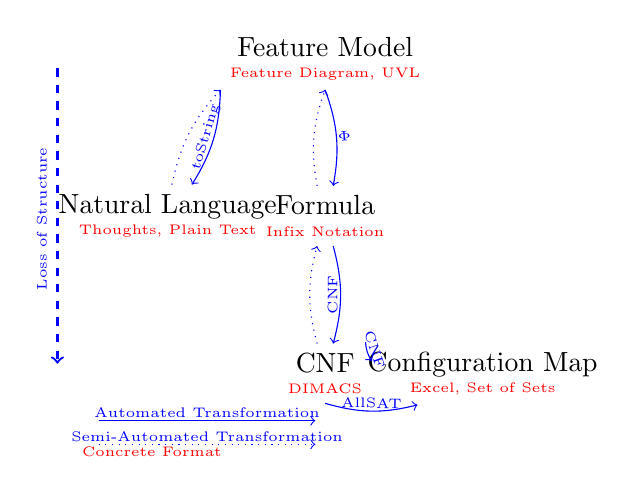
\begin{tikzpicture}
			\tikzstyle{every edge}=[font=\tiny,draw,color=blue]

			\node (topleft) at (-1.4,0) {};
			\node (bottomleft) at (-1.4,-4) {};
			
			\node (fd) at (2,0) [align=center] {Feature Model\\[-1ex]{\tiny\color{red}Feature Diagram, UVL}};
			\node (nat) at (0,-2) [align=center] {Natural Language\\[-1ex]{\tiny\color{red}Thoughts, Plain Text}};
			\node (phi) at (2,-2) [align=center] {Formula\\[-1ex]{\tiny\color{red}Infix Notation}};
			\node (cfg) at (4,-4) [align=center] {Configuration Map\\[-1ex]{\tiny\color{red}Excel, Set of Sets}};
			\node (cnf) at (2,-4) [align=center] {CNF\\[-1ex]{\tiny\color{red}DIMACS}};

			\path [dashed, thick, ->] (topleft) edge node[left, rotate=90, yshift=2mm, xshift=10mm] {Loss of Structure} (bottomleft);
		
			\path [->] (fd.south west) edge[bend left=15] node[sloped,yshift=1mm] {toString} (nat);
			\path [dotted, ->] (nat) edge[bend left=15] node[sloped,yshift=1mm] {} (fd.south west);
			
			\path [->] (fd.south) edge[bend left=15] node[sloped,yshift=1mm,rotate=90] {$\Phi$} (phi);
			\path [dotted, ->] (phi) edge[bend left=15] node[sloped,yshift=2mm,rotate=270] {} (fd.south);

			\path [->] (phi) edge[bend left=15] node[sloped,yshift=1mm] {CNF} (cnf);
			\path [dotted, ->] (cnf) edge[bend left=15] node[sloped,yshift=2mm,rotate=270] {} (phi);
		
			\path [->] (cfg) edge[bend right=15] node[sloped,yshift=1mm] {CNF} (cnf);
			\path [->] (cnf.south) edge[bend right=15] node[sloped,yshift=1mm] {AllSAT} (cfg);

			\node (trans) at (-1,-4.6) {};
			\node (trans2) at (2,-4.6) {};
			\node (trans3) at (-1,-4.9) {};
			\node (trans4) at (2,-4.9) {};
			\path [->] (trans) edge node[yshift=1mm] {Automated Transformation} (trans2);
			\path [dotted, ->] (trans3) edge[yshift=5mm] node[yshift=1mm] {Semi-Automated Transformation} (trans4);
		
			\node (bottomleft2) at (-0.2,-5) {\tiny\color{red}Concrete Format};
		\end{tikzpicture}
	\end{mycolumns}
\end{frame}

\subsubsection{Features}

\begin{frame}{\myframetitle}
	\begin{mycolumns}[t]
		\emph{Consistency of Features (SAT)}
		\mydefinition{Core/Dead Feature}{
			\begin{itemize}
				\item can a feature $F$ be (de-)selected at all?
			\end{itemize}
			\centering
			\begin{tikzpicture}
				\tikzset{block/.style={align=center,minimum height=5mm}}
				\node [block] (query) {$\phi \pand F$};
				\node [block, right =10mm of query] (answer) {$\bot/\top$};
				\node [block, above right =-3mm and 6mm of answer] (void) {$F$ is \emph{dead}};
				\node [block, below right =-3mm and 6mm of answer] (notvoid) {$F$ is not dead};
				\path[draw,->,color=blue] (query) edge node[yshift=2mm] {\small SAT} (answer)
							(answer) edge node [yshift=2mm,sloped]{\small $\bot$} (void)
							(answer) edge node [yshift=-2mm,sloped]{\small $\top$} (notvoid);
			\end{tikzpicture}
			\begin{tikzpicture}
				\tikzset{block/.style={align=center,minimum height=5mm}}
				\node [block] (query) {$\phi \pand \pnot F$};
				\node [block, right =10mm of query] (answer) {$\bot/\top$};
				\node [block, above right =-3mm and 6mm of answer] (void) {$F$ is \emph{core}};
				\node [block, below right =-3mm and 6mm of answer] (notvoid) {$F$ is not core};
				\path[draw,->,color=blue] (query) edge node[yshift=2mm] {\small SAT} (answer)
							(answer) edge node [yshift=2mm,sloped]{\small $\bot$} (void)
							(answer) edge node [yshift=-2mm,sloped]{\small $\top$} (notvoid);
			\end{tikzpicture}
		}
		\mynextcolumn
		\emph{Cardinality of Features (\ssat{})}
		\mydefinition{How Many Products Include Feature $F$?}{
			\centering
			\begin{tikzpicture}
				\tikzset{block/.style={align=center,minimum height=5mm}}
				\node [block] (query) {$\phi \pand F$};
				\node [block, right =10mm of query] (answer) {$\abs{\{S \in C \mid F \in S\}}$};
				\path[draw,->,color=blue] (query) edge node[yshift=2mm] {\small \ssat{}} (answer);
			\end{tikzpicture}
		}
		\mydefinition{Commonality: How Dead is This Feature?}{
			\centering
			\begin{tikzpicture}
				\tikzset{block/.style={align=center,minimum height=5mm}}
				\node [block] (query) {$\phi \pand F$};
				\node [block, right =7mm of query] (answer) {$\abs{\{S \in C \mid F \in S\}}$};
				\node [block, right =2mm of answer] (num) {$\frac{\abs{\{S \in C \mid F \in S\}}}{\abs{C}}$};
				\path[draw,->,color=blue] (query) edge node[yshift=2mm] {\small \ssat{}} (answer)
							(answer) edge node [yshift=2mm,sloped]{} (num);
			\end{tikzpicture}
		}
	\end{mycolumns}
	\begin{mycolumns}[t]
		\myexampletight{}{
			\centering
			{\small\featureDiagram{Root,concrete[X,concrete,alternative][Y,concrete]}\\$\pnot X$}

			$X$ is dead, $Root$ and $Y$ are core
		}
		\mynextcolumn
		\myexampletight{}{
			\centering
			{\small\featureDiagram{Root,concrete[X,concrete,alternative][Y,concrete]}\\$\pnot X$}

			$X$: 0 products, $Root$ and $Y$: 1 products
		}
	\end{mycolumns}
\end{frame}

\subsubsection{Partial Configurations}

\begin{frame}{\myframetitle}
	\begin{mycolumns}[t]
		\emph{Consistency of Partial Configurations (SAT)}
		\mydefinition{Valid Partial Configuration}{
			\begin{itemize}
				\item does a partial configuration $C = ({\color{green}S}, {\color{red}D})$ contain a mistake?
			\end{itemize}
			\centering
			\begin{tikzpicture}
				\tikzset{block/.style={align=center,minimum height=5mm}}
				\node [block] (query) {$\phi \pand \bigwedge_{s \in S} {\color{green}s} \pand \bigwedge_{d \in D} {\color{red}\pnot d}$};
				\node [block, right =10mm of query] (answer) {$\bot/\top$};
				\node [block, above right =-3mm and 6mm of answer] (void) {$C$ $\times$};
				\node [block, below right =-3mm and 6mm of answer] (notvoid) {$C$ \checkmark};
				\path[draw,->,color=blue] (query) edge node[yshift=2mm] {\small SAT} (answer)
							(answer) edge node [yshift=2mm,sloped]{\small $\bot$} (void)
							(answer) edge node [yshift=-2mm,sloped]{\small $\top$} (notvoid);
			\end{tikzpicture}
		}
		\mynextcolumn
		\emph{Cardinality of Partial Configurations (\ssat{})}
		\mydefinition{How Many Products Are Still Configurable for $C$?}{
			\centering
			\begin{tikzpicture}
				\tikzset{block/.style={align=center,minimum height=5mm}}
				\node [block] (query) {$\phi \pand ...$};
				\node [block, right =10mm of query] (answer) {$\abs{\{(S', D') \in C \mid {\color{green}S} \subseteq S', {\color{red}D} \in D'\}}$};
				\path[draw,->,color=blue] (query) edge node[yshift=2mm] {\small \ssat{}} (answer);
			\end{tikzpicture}
		}
	\end{mycolumns}
	\begin{mycolumns}[t]
		\myexampletight{}{
			\centering
			{\small\featureDiagram{Root,concrete[X,concrete,optional][Y,concrete,optional]}\\$X \pimplies Y$}

			\cfg{Root}{X} \checkmark
		}
		\mynextcolumn
		\myexampletight{}{
			\centering
			{\small\featureDiagram{Root,concrete[X,concrete,optional][Y,concrete,optional]}\\$X \pimplies Y$}

			\cfg{Root}{X}: 2 products
		}
	\end{mycolumns}
\end{frame}

\subsection{Automated Analyses in FeatureIDE}

\subsubsection*{Feature-Model Editor}

\begin{frame}{\myframetitle}
	\begin{mycolumns}[widths={60,40}]
		\myexampletight{}{
			\pic[width=\textwidth]{featureide-feature-model-editor-waffle}
		}
	\mynextcolumn
		\myexampletight{}{
			\pic[width=\textwidth]{featureide-feature-model-statistics}
		}
	\end{mycolumns}
\end{frame}

\subsubsection*{Configuration Editor}

\begin{frame}{\myframetitle}
	\begin{mycolumns}[widths={60,40}]
		\myexampletight{}{
			\centering
			\pic[width=.27\textwidth]{featureide-configuration-editor-step1}
			$\Rightarrow$
			\pic[width=.63\textwidth]{featureide-configuration-editor-step2}
		}
	\mynextcolumn
		\mynote{Decision Propagation}{
			\begin{itemize}
				\item after each decision (i.e., click) \ldots
				\begin{itemize}
					\item \ldots{} select features that are now \emph{conditionally core}
					\item \ldots{} deselect features that are now \emph{conditionally dead}
				\end{itemize}
				\item this way it is impossible to configure an invalid product
				\item explanations for all propagated decisions
			\end{itemize}
		}
	\end{mycolumns}
\end{frame}

\begin{frame}{Automated Analysis of Feature Models}
	\begin{mycolumns}
		\mydefinition{The Road So Far \ldots}{
			\centering
			\begin{tikzpicture}
				\tikzset{block/.style={align=center,minimum height=5mm}}
				\node [block] (fm) {Feature Model};
				\node [block, right =4mm of fm] (formula) {Formula};
				\node [block, right =8mm of formula] (cnf) {DIMACS};
				\node [block, below right =8mm and -12mm of fm] (query) {Query};
				\node [block, below =-.5mm of query,align=center,color=blue,font={\footnotesize}] (query2) {void feature model\\variability factor\\all products\\core/dead features\\false-optional features\\commonality\\valid partial configuration\\decision propagation};
				\node [block, right =27mm of query] (answer) {Answer};
				\node [block, right =4mm of answer] (result) {};
				\node [coordinate, below right =5mm and 2mm of cnf] (right) {};
				\node [coordinate, above left =3mm and 2mm of query] (left) {};
				\path[draw,->,color=blue] (fm) edge node[yshift=2mm] {\small $\Phi$} (formula)
							(formula) edge node[yshift=2mm,align=center] {\small $CNF$} (cnf)
							(cnf.east) -| (right) -- node[yshift=2mm] {\small formulate} (left) |- (query)
							(query) edge node[yshift=-2mm,align=center,font={\footnotesize}] {{\small solve}\\[1.5ex]SAT\\\ssat{}\\AllSAT} (answer)
							(answer) edge (result);
			\end{tikzpicture}
		}
	\mynextcolumn
		\mydefinition{\ldots and Beyond}{
			\centering
			\begin{tikzpicture}
				\tikzset{block/.style={align=center,minimum height=5mm}}
				\node [block,align=center,color=red,font={\footnotesize}] (fm2) {attributes\\cardinalities\\submodels};
				\node [block, below =.5mm of fm2] (fm) {Feature Model};
				\node [block, right =4mm of fm] (formula) {Formula};
				\node [block, above =.5mm of formula,align=center,color=red,font={\footnotesize}] (formula2) {quantifiers\\predicates\\functions};
				\node [block, right =8mm of formula] (cnf) {DIMACS};
				\node [block, above =.5mm of cnf,align=center,color=red,font={\footnotesize}] (cnf2) {DNF\\d-DNNF\\BDD};
				\node [block, below right =8mm and -12mm of fm] (query) {Query};
				\node [block, below =-.5mm of query,align=center,color=red,font={\footnotesize}] (query2) {atomic sets\\redundant constraints\\feature-model edits\\explanations\\sampling\\slicing};
				\node [block, right =27mm of query] (answer) {Answer};
				\node [block, right =4mm of answer] (result) {};
				\node [coordinate, below right =5mm and 2mm of cnf] (right) {};
				\node [coordinate, above left =3mm and 2mm of query] (left) {};
				\path[draw,->,color=blue] (fm) edge node[yshift=2mm] {\small $\Phi$} (formula)
							(formula) edge node[yshift=0mm,align=center] {\small $CNF$\\{\footnotesize\color{red}Tseitin}} (cnf)
							(cnf.east) -| (right) -- node[yshift=2mm] {\small formulate} (left) |- (query)
							(query) edge node[yshift=-7mm,align=center,font={\footnotesize}] {{\small solve}\\[1.5ex]SAT, \ssat{}, AllSAT\\{\color{red}MAX-SAT}\\{\color{red}Solution-SAT}\\{\color{red}MUS}\\{\color{red}SMT, CSP}\\{\color{red}QBF}\\{\color{red}WMC, PMC}} (answer)
							(answer) edge (result);
			\end{tikzpicture}
			\vspace*{-4ex}
			\begin{itemize}
				\item develop new analyses
				\item improve efficiency of existing analyses
				\item investigate correctness and compositionality
			\end{itemize}
		}
	\end{mycolumns}
\end{frame}

\lessonslearned{
	\item Automated SAT-based analyses help in understanding large configuration spaces.
	\item There are still many open problems regarding encodings and applications (e.g., \#SAT).
}{
	\item David Benavides et al. (2010): \href{https://doi.org/10.1016/j.is.2010.01.001}{Automated Analysis of Feature Models 20 Years Later: A Literature Review}
	\item Thomas Thüm et al. (2009): \href{https://doi.org/10.1109/ICSE.2009.5070526}{Reasoning About Edits to Feature Models}
	\item Chico Sundermann et al. (2021): \href{https://doi.org/10.1145/3442391.3442404}{Applications of \#SAT Solvers on Feature Models}
}{
	% alternative: find inconsistencies in your feature diagram
	\item Recall that some $f \in F$ is dead iff $\pnot SAT(\phi \pand f)$.
	Suppose you want to know \emph{all} dead features of $\phi$.
	Naively, you may formulate $\abs{F}$ SAT queries.
	
	Can this be improved?
	
	(Hint: Some SAT solvers return an example model $M_\psi$ when $\psi$ is satisfiable.)
}

\mode<beamer>{
	\begin{frame}{\inserttitle}
		\lectureseriesoverview
	\end{frame}

	\contentoverview
}


\end{document}
